\chapter{Results}

\section{Patients' Demographics}

This study included a cohort of 30 patients with advanced NSCLC from whom a total of 39 samples were extracted, 37 of plasma and 2 of cerebrospinal fluid (CSF). Within the plasma samples, 24 (64.9\%) were cfDNA-based liquid biopsies and 13 (35.1\%) were drawn for exosome isolation.

Patients' clinicopathological information at the time of the liquid biopsies sampling is summarized in \autoref{tab:Patients}. The median age was 54 years (range: 36–81), with a uniform distribution of females (N$=$17) and males (N$=$13). Most of the patients were never smokers (60\%), which is in accordance with the ALK-positive NSCLC characteristics, 8 were former smokers (26.7\%), and 4 were current smokers (13.3\%). All the individuals underwent a successful histological examination, which revealed that the majority presented an adenocarcinoma (93.3\%), and the remaining 2 cases a neuroendocrine carcinoma (6.7\%). Furthermore, most of them were classified as patients with stage IV (76.7\%) and stage III (20\%) disease. Treatment procedures were performed in 6 different hospitals across Spain using the main ALK inhibitors, except for 2 cases that were on chemotherapy and 2 that had no associated treatment. In this context, 16 patients were receiving second-generation ALK inhibitors such as alectinib (36.7\%), ceritinib (13.3\%), and brigatinib (3.3\%), while 9 were administered the first-generation ALK inhibitor crizotinib (30\%). The remaining patient was prescribed the third-generation inhibitor lorlatinib (3.3\%). Regarding their ECOG performance status, it ranged from 0 (N$=$14) to 1 (N$=$13). Therefore, a large part of the cohort was asymptomatic at the time of sample drawing, and another part had symptoms restricting them from physically strenuous activities.

\begin{table}[t]
\centering
\resizebox{0.65\textwidth}{!}{
\renewcommand{\arraystretch}{1.25}
\begin{tabular}{cccc}
\rowcolor[HTML]{C0C0C0} 
\textbf{Clinical feature} & \textbf{Grouping}  & \textbf{N} & \textbf{\%} \\
\rowcolor[HTML]{FFFFFF}
\textbf{Age of diagnosis} & Median & 54 & - \\
\rowcolor[HTML]{EFEFEF}
\cellcolor[HTML]{EFEFEF} & Female & 17 & 56.7\% \\
\rowcolor[HTML]{EFEFEF}
\multirow{-2}{*}{\cellcolor[HTML]{EFEFEF}\textbf{Sex}} & Male & 13 & 43.3\% \\
\rowcolor[HTML]{FFFFFF}
\cellcolor[HTML]{FFFFFF} & Never smokers & 18 & 60\% \\
\rowcolor[HTML]{FFFFFF}
\cellcolor[HTML]{FFFFFF} & Former smokers & 8 & 26.7\% \\
\rowcolor[HTML]{FFFFFF}
\multirow{-3}{*}{\cellcolor[HTML]{FFFFFF}\textbf{Smoking status}} & Current smokers & 4 & 13.3\% \\
\rowcolor[HTML]{EFEFEF}
\cellcolor[HTML]{EFEFEF} & 0 & 14 & 46.7\% \\
\rowcolor[HTML]{EFEFEF}
\cellcolor[HTML]{EFEFEF} & 1 & 13 & 43.3\% \\
\rowcolor[HTML]{EFEFEF}
\multirow{-3}{*}{\cellcolor[HTML]{EFEFEF}\textbf{\begin{tabular}[c]{@{}c@{}}ECOG\\ performance status\end{tabular}}} & 2 & 3 & 10\% \\
\rowcolor[HTML]{FFFFFF}
\cellcolor[HTML]{FFFFFF} & Adenocarcinoma & 28 & 93.3\% \\
\rowcolor[HTML]{FFFFFF}
\multirow{-2}{*}{\cellcolor[HTML]{FFFFFF}\textbf{Histology}} & Neuroendocrine carcinoma & 2 & 6.7\% \\
\rowcolor[HTML]{EFEFEF} 
\cellcolor[HTML]{EFEFEF} & IV & 23 & 76.7\% \\
\rowcolor[HTML]{EFEFEF}
\cellcolor[HTML]{EFEFEF} & III & 6 & 20\% \\
\rowcolor[HTML]{EFEFEF}
\multirow{-3}{*}{\cellcolor[HTML]{EFEFEF}\textbf{\begin{tabular}[c]{@{}c@{}}Initial\\ clinical stage\end{tabular}}}  & II & 1 & 3.3\% \\
\rowcolor[HTML]{FFFFFF}
\cellcolor[HTML]{FFFFFF} & Alectinib & 11 & 36.7\% \\
\rowcolor[HTML]{FFFFFF}
\cellcolor[HTML]{FFFFFF} & Crizotinib & 9 & 30\% \\
\rowcolor[HTML]{FFFFFF}
\cellcolor[HTML]{FFFFFF} & Ceritinib & 4 & 13.3\% \\
\rowcolor[HTML]{FFFFFF}
\cellcolor[HTML]{FFFFFF} & Chemotherapy & 2 & 6.7\% \\
\rowcolor[HTML]{FFFFFF}
\cellcolor[HTML]{FFFFFF} & No treatment & 2 & 6.7\% \\
\rowcolor[HTML]{FFFFFF}
\cellcolor[HTML]{FFFFFF} &  Brigatinib & 1 & 3.3\% \\
\rowcolor[HTML]{FFFFFF}
\multirow{-7}{*}{\cellcolor[HTML]{FFFFFF}\textbf{Treatment}} & Lorlatinib & 1 & 3.3\%
\end{tabular}}
\caption{Clinicopathological characteristics of the study population (N$=$30) at the time of the sample collection.}
\label{tab:Patients}
\end{table}

Finally, it should be mentioned that in this study a subject was considered as two different patients if progression to a specific treatment was observed in that patient, that is if another sample was obtained and sequenced with the patient receiving different treatment than the initial one. On the other hand, patients with multiple sequenced samples but with the same treatment were counted as a single one. In this context, this study had 27 unique individuals, 3 of them progressing to an ALK inhibitor.

\section{Next Generation Sequencing Performance}

The liquid biopsy samples from each of the patients were analyzed using NGS, which identified genetic mutations according to the wide range of hotspots in key genes addressed by the Oncomine\texttrademark{} Pan-Cancer Cell-Free Assay.

For this study, 39 samples were sequenced using 9 different NGS runs. On average, the percentage of chip wells that contained an ISP was 85.0\%, resulting in 53.4\% of usable sequences (library ISPs that passed the polyclonal, low quality, and primer dimer filters). These called reads had an average length of 76.8 $bp$. The average of mapped reads per sample was about 9.1 million, while its mean sequencing depth was 25050 reads. Regarding the coverage uniformity, it was higher than 74.0\% in all the analyzed samples.

Under these conditions, more than 170 potentially malignant mutations in genes such as ALK, EGFR, KRAS, TP53, PIK3CA, FGFR1, or PDGFRA, among others, were initially accounted. From this set, 84 of the alterations involved the ALK gene. Each of these possible mutations was manually filtered as described in \autoref{sec:Secondary_analysis}. As a result of this assessment, 67.9\% of the initial ALK variants were excluded from further analysis. In this context, 27 potential ALK alterations were finally identified from 18 different samples (17 patients), which were subsequently verified by digital PCR.

On the other hand, taking into account the clinical interest of pathological mutations, 7 additional samples from 6 different patients were also confirmed by dPCR since their characteristics (molecular coverage, read counts, etc.) made them susceptible to being positive. These samples included mutations in the EGFR, KRAS, TP53, and PIK3CA genes.

Finally, it should be noted that all the selected samples had a MAF above the limit of detection (0.1\%).

\section{Mutational Spectrum}

% Additionally, highly represented mutations without a clear pathological influence and confirmed by the secondary analysis carried out in \autoref{sec:Secondary_analysis} have also been included in the final results.

% decir que se han confirmado por igv algunas mutaciones 

% ALK white type 22

% 7 pacientes no presentaban ninguna mutación
% 1 paciente solo con ALK
% 7 pacientes con ALK + TP53
% 12 pacientes solo con TP53
% 1 paciente con PIK3CA + TP53
% 1 paciente PIK3CA
% 1 paciente con FGFR1 + KRAS + TP53 > no va a haber alk aquí
 
% ALK: 8 missenses
% FGFR1: 1 indel
% KRAS: 1 messense
% PIK3CA: 2 missenses
% TP53: 
%     2 indels
%     8 missenses
%     11 multiple mutations
%         22 missenses
%         9 indels

% Paper nuevo
% Overall, somatic variants in ctDNA were detected in 24  patients. There were no significant differences in cfDNA input between patients in whom a somatic mutation was detected in the cfDNA and those in whom it was not (n=2).  The average number of mutations per patient was 4.1 and median MAF was XX%. As expected, the most frequent mutation type was single-nucleotide polymorphisms (SNVs) (n = 97).  In addition, we identified 7 indels and three CNVs (Figure 1). Specifically a c-MYC gain along with a CCND1 and a FGFR3 loss were detected in the same patient.  Using this Pan-Cancer Cell-Free Assay, somatic mutations were detected in 10 genes. TP53 was the most frequently mutated gene, followed by FGFR2, GNAQ, IDH1, ALK and CCND3. A complete list of all variants detected is available in Supplemental table 2. 


% cclm
% ctDNA collected at the time of disease progression was available from seven patients for NGS analysis. In this subset of patients, PIK3CA mutations were the alterations most frequently detected upon disease progression, being found in four patients. 

% CCLM
% Among the total 61 mutations detected by the OncomineTM Lung cfDNA Assay kit, we were able to perform 54 confirmations by dPCR (88.5%) using both custom TaqMan® assays and predesigned TaqMan® assays.
% Altogether, 34 out of 36 patients with an NGS-positive result were deemed evaluable for confirmation analysis between NGS and dPCR. This cohort had a total of 54 mutations detected by NGS. Of these, 49 were also detected by dPCR (89%).
%Five mutations were reported exclusively by NGS, which corresponded to samples in which mutations were detected at MAF close to NGS and dPCR LOD (MAF ≤ 0.1%)...

% https://www.ncbi.nlm.nih.gov/pmc/articles/PMC5039376/
% The MAFs were all higher than the LOD of the ddPCR platform, therefore ruling out the possibility of false positive
% Mutant allele concentration (copies/µl, CMUT) and wild-type allele concentration (copies/µl, CWT) were calculated and mutant allele frequency (MAF) was calculated as: MAF = CMUT/(CMUT + CWT).

% https://books.google.es/books?id=gijVCwAAQBAJ&pg=PT745&lpg=PT745&dq=maf+dpcr&source=bl&ots=UEBSZFWsnN&sig=ACfU3U3uL_R6J0ew8rOUbOAJqao0Y8e0kg&hl=es&sa=X&ved=2ahUKEwi2-fiJ5PvpAhVP6RoKHekZD_QQ6AEwAHoECAoQAQ#v=onepage&q&f=false
% Mutations could be robustly detected in plasma samples using dPCR with a sensitivity as low as 0.1% and a sensitivity of 0.5% using NGS. All mutations previously identified using NGS were validated using dPCR in tumor (n=27) as well as in plasma samples (n=5).
%Moreover, dPCR identified 4 additional mutations in 4 plasma samples in the neoadjuvant setting and 4 in the metastatic setting, 2 in tumor and 2 in plasma samples. The mutant allelic frequencies (MAF) of these newly identified mutations were very low (range 0.2%-1.8%) close to the detection limit of the technology. Through the use of dPCR, the detection rate of plasma ctDNA increased from 8% using NGS to 38% in the neoadjuvant setting and from 67% using NGS to 100% in the metastatic setting thereby highlighting the greater sensitivity of the dPCR technology.
% The MAF assessed by NGS and dPCR were highly correlated both in the neoadjuvant and metastatic (Spearman p=0.84 and p=0.97) settings, a higher concordance between NGS and dPCR being observed when the MAF are high.
%Conclusions: The use of dPCR allows the detection of low-frequency tumor-specific mutations in plasma with a greater sensitivity compared to NGS providing the high accuracy and sensitivity essential for liquid biopsies.

% https://www.ncbi.nlm.nih.gov/pmc/articles/PMC6225899/
% In ALK-rearranged NSCLC co-occurring TP53 mutations predict an unfavorable outcome of systemic therapy.

% NSCLC_alterations
% Furthermore, tumours bearing co-mutations in TP53 exhibit higher degrees of copy number genomic instability (aneuploidy) and a higher somatic mutation burden. Therefore, TP53 co-mutations impact the natural history of EGFR-mutant NSCLC at least partially by allowing tolerance of a greater degree of genomic instability, which results in both larger numbers of co-occurring truncal drivers and late subclonal diversification with focal emergence of high-amplitude amplifications and deletions in mediators of therapeutic resistance104. In keeping with a more complex genomic landscape and a larger burden of clonal or subclonal co-drivers, multiple clinical studies have identified TP53 co-alterations as a negative prognostic marker in EGFR-mutant LUAD and a consistent predictor of worse clinical outcomes following EGFR TKI therapy

% CCLM
% Most mutations identified were single-nucleotide polymorphisms (n = 49). We also detected deletions (n = 11) and one insertion (Supplemen- tary Table 3).
% Interestingly, the resistance mutation to ALK inhibitors, p.G1269A in the kinase domain of ALK, was found in two ALK-positive NSCLC patients who had progressed on crizotinib (Figure 2). 

% Todos estos resultados fueron utilizados posteriormente para establecer los parámetros del algoritmo implementado.



%\begin{figure}[ht]
%    \centering
%    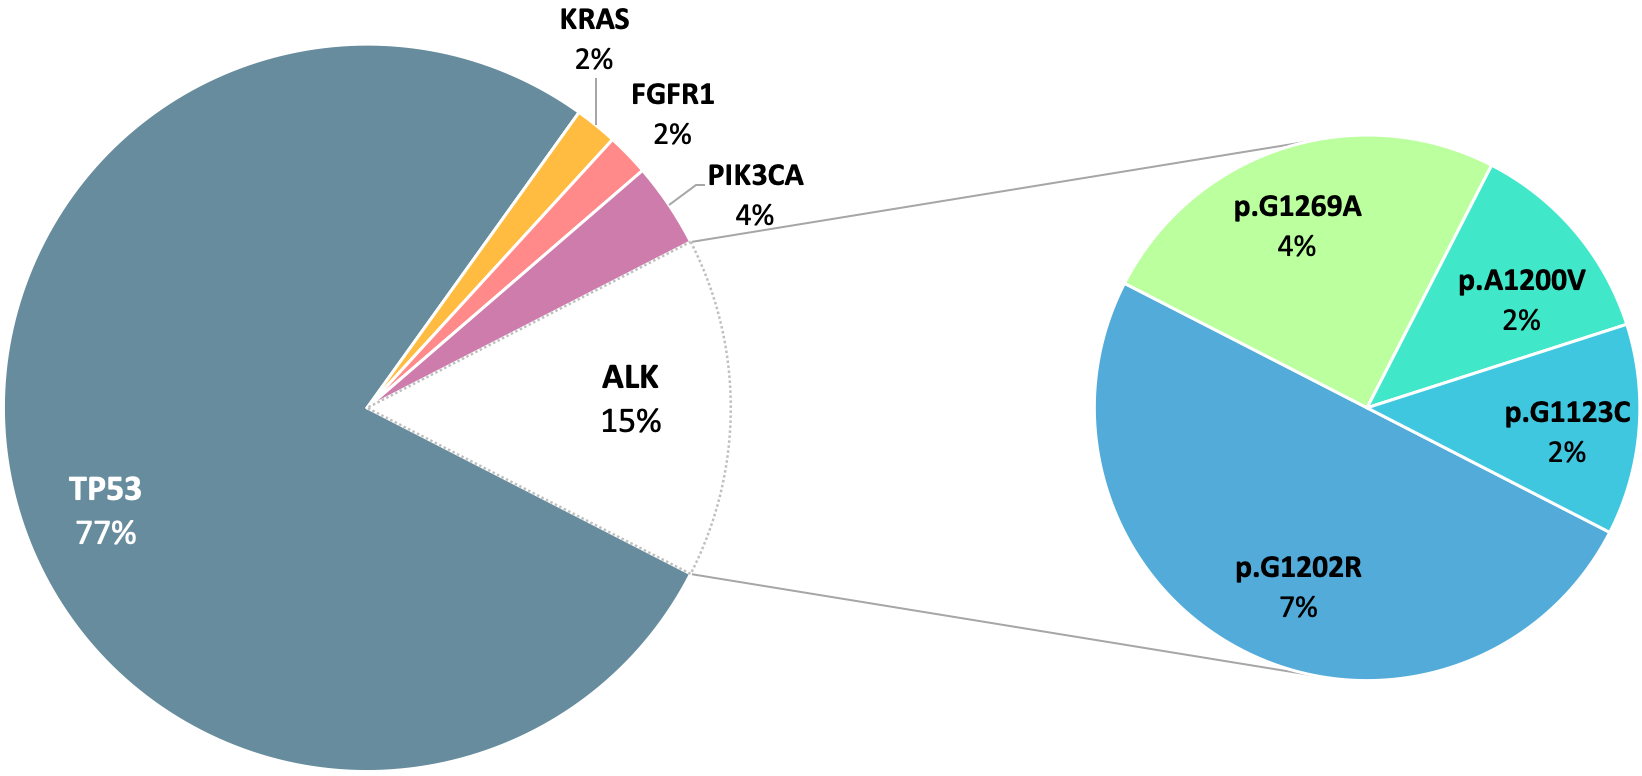
\includegraphics[width=0.88\textwidth]{Images/chapter_4/all_mutations.png}
%    \caption{Frequency of the mutations identified in the study population, as well as the the different types of missense mutations detected in the ALK gene.}
%    \label{fig:All_mutations}
%\end{figure}

% 53 mutations were identified after analyzing and manually filtering (as described in \autoref{sec:Secondary_analysis}) the variants obtained from the sequencer. As reflected in \autoref{fig:All_mutations}, the most widely represented mutations occurred in the TP53 gene, with 41 cases. In fact, it was common to find multiple alterations of this type in the same sample. ALK mutations, which are the target of this study, were identified in 8 samples. On the other hand, alterations were also detected in the PIK3CA, KRAS, and FGFR1 genes, appearing both individually and coexisting with the rest of the detected variants.

\section{Implemented Pipeline}

The development of the bioinformatic pipeline was divided into two steps: the implementation of the filtering algorithm itself; and that of a graphical interface to simplify the process of selecting parameters and saving the output variants along with their properties in a \textit{.csv} file.

\subsection{Algorithm Characterization}

In order to detect all variants at the ALK gene locus, specific conditions for each of them were established from a set of previously validated samples. The flowchart in \autoref{fig:Algorithm} shows the basic structure of the developed pipeline and the selection criteria based on certain variables as presented in the \textit{non-filtered-oncomine.tsv} file.

\begin{figure}[ht]
    \centering
    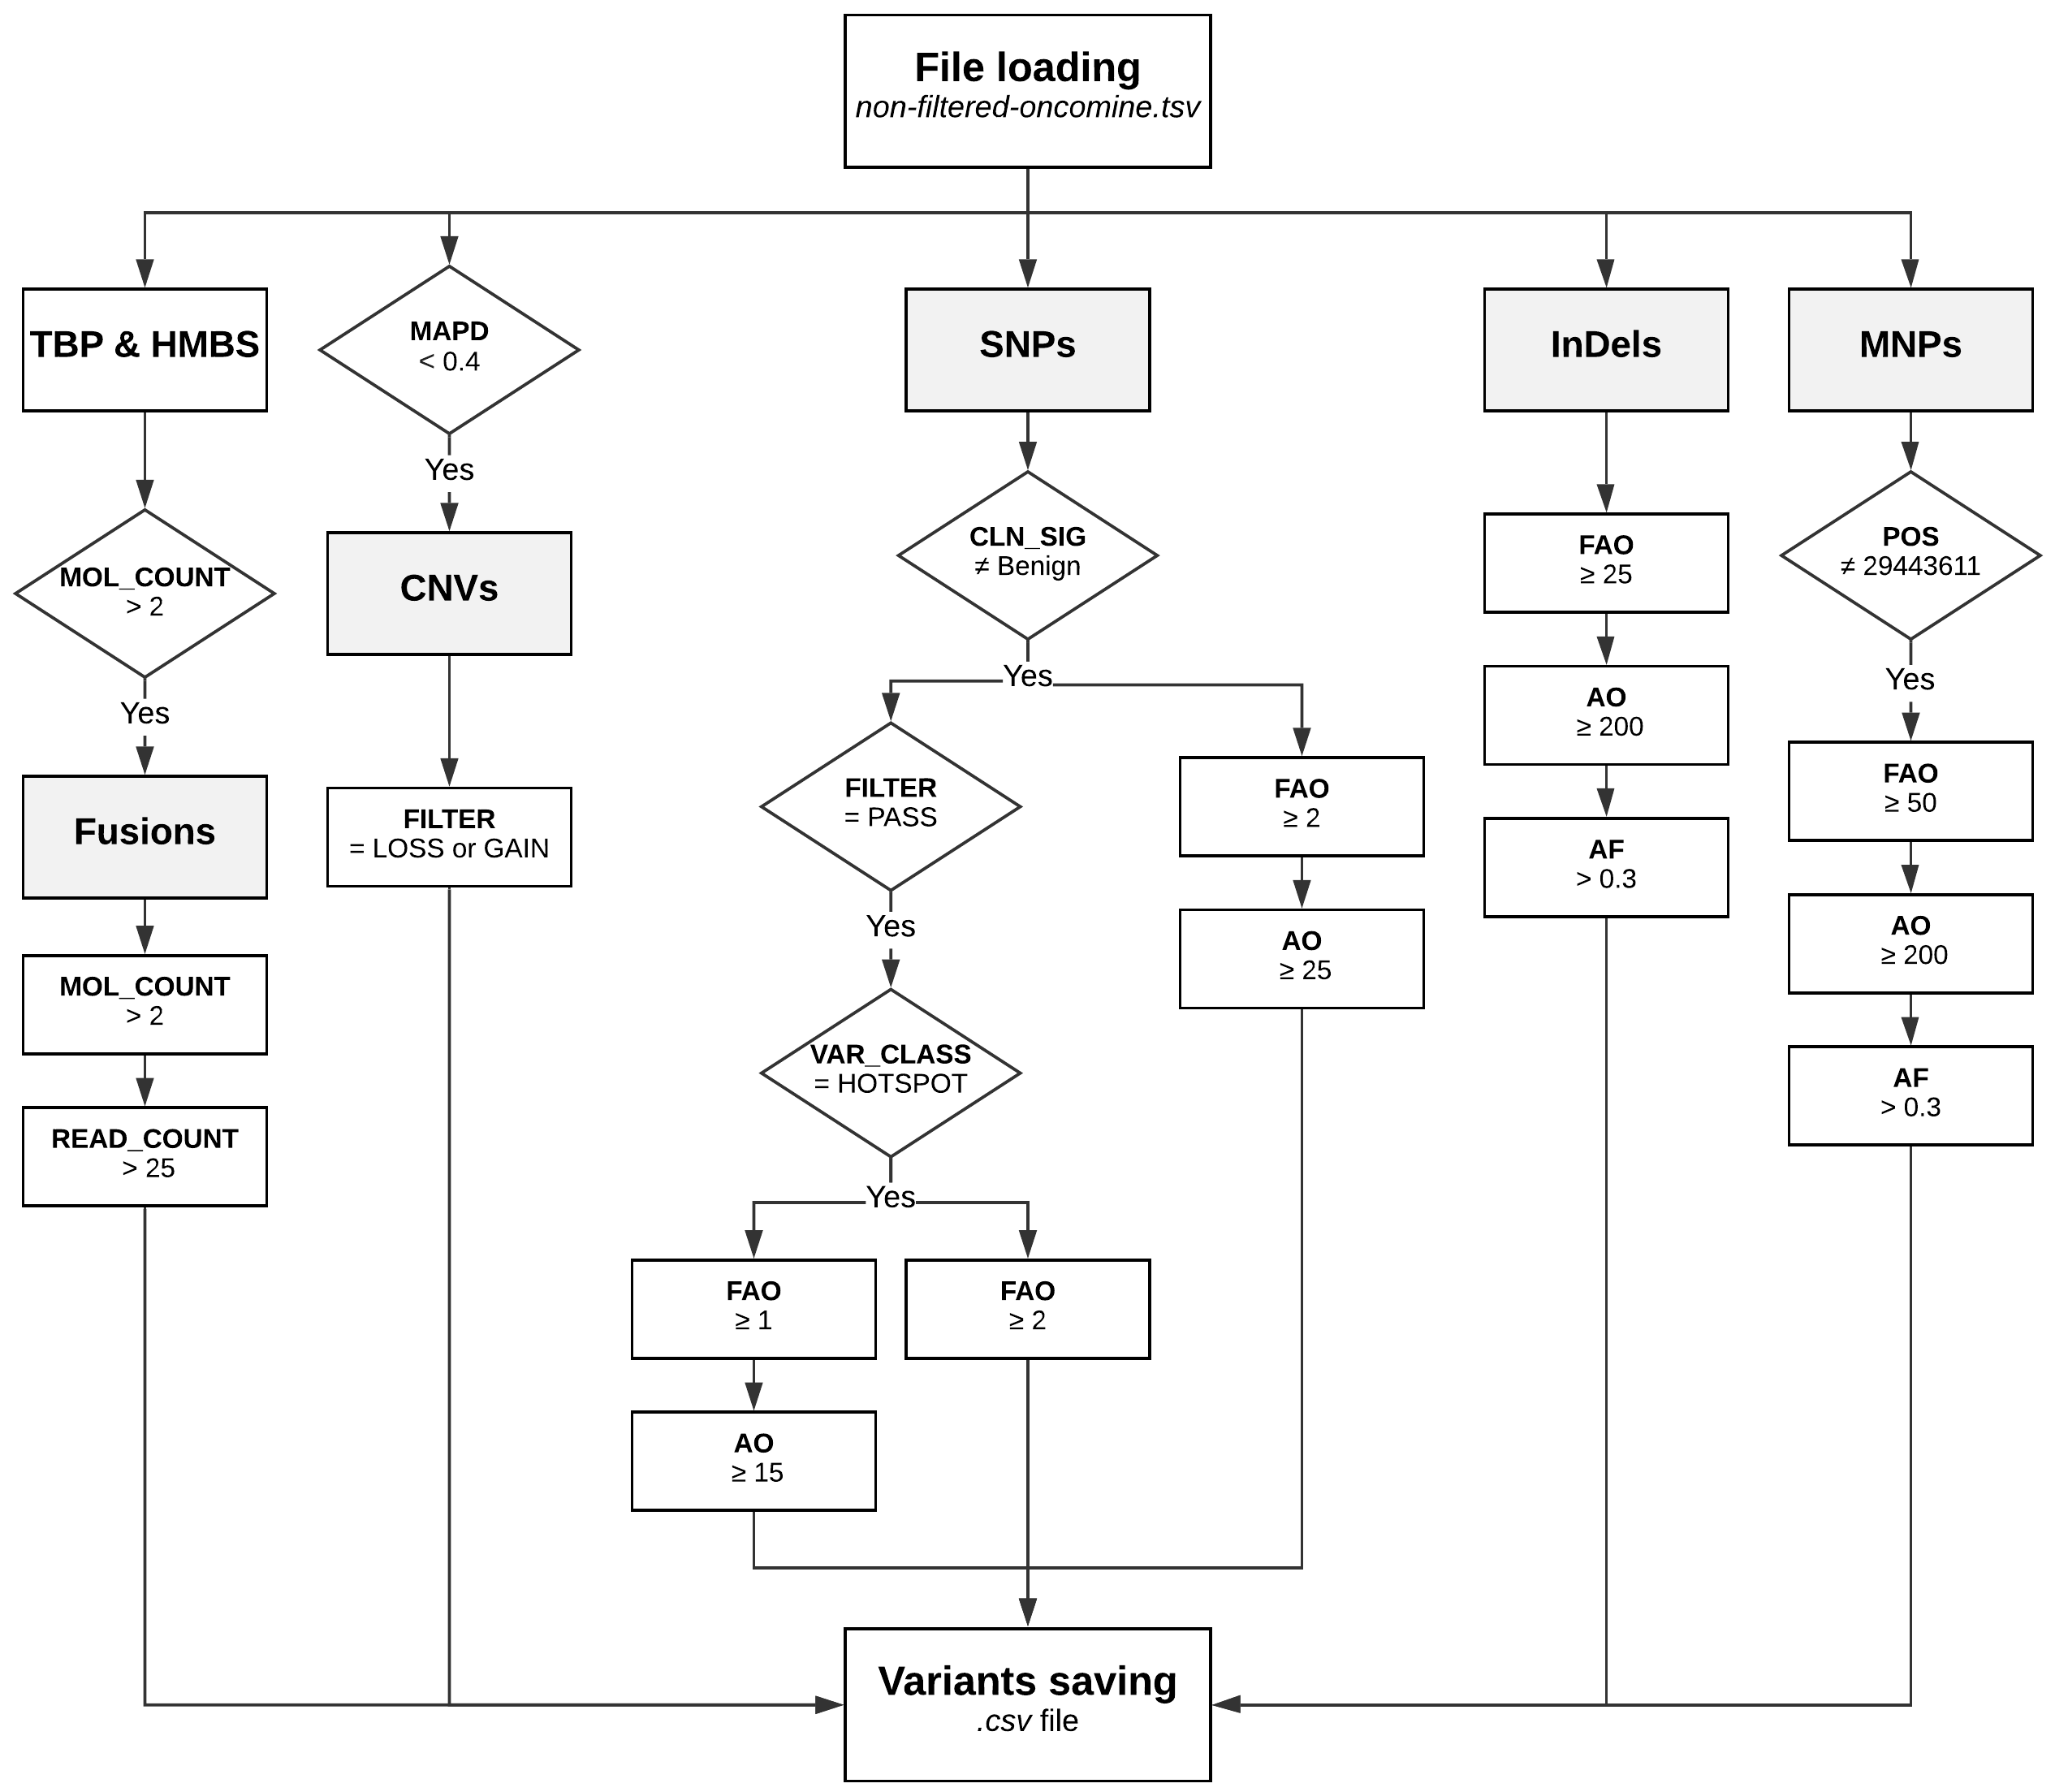
\includegraphics[width=\textwidth]{Images/chapter_4/mut_filtering.png}
    \caption{Flowchart of the bioinformatic pipeline optimized for the processing and assessment of variants at the ALK gene locus. MOL\_COUNT, molecular coverage; READ\_COUNT, read coverage; MAPD, median of the absolute values of all pairwise differences; FILTER: Ion Reporter\texttrademark{} internal filter (Oncomine\texttrademark{} Variants v5.12); CLN\_SIG, clinical significance; VAR\_CLASS: Oncomine\texttrademark{} Variant Class; POS: variant position; AF, allele frequency.}
    \label{fig:Algorithm}
\end{figure}

\subsubsection{Fusions Filtering}

The fusions filter selects translocations at the ALK locus with molecular coverage $> 2$, and fusion reads $> 25$. These thresholds were established according to the clinical study data and the Oncomine\texttrademark{} Pan‐Cancer Cell‐Free Assay recommendations.

Additionally, two control genes were included in each sequencing process to measure the transcript abundance, TATA-binding protein (TBP) and hydroxymethylbilane synthase (HMBS). Both must have molecular coverage $> 2$ to validate the filtered fusion variants by ensuring their correct amplification.

\subsubsection{Copy-Number Variations Filtering}

Following the Ion Reporter\texttrademark{} recommendations, to make a CNV call the median of the absolute values of all pairwise differences (MAPD) must be $< 0.4$. MAPD measures the absolute difference between the $log_2$ copy-number ratios of adjacent amplicons and then calculates the median across all wells (\autoref{eq:MAPD}).
\begin{align} \label{eq:MAPD}
    MAPD &= median(\mid x_{i+1}-x_i \mid) \\
    \text{where}~
    x_i &\equiv \text{$log_2$ ratio for marker i} \notag
\end{align}

Larger MAPD values indicate lower coverage uniformity and greater noise, resulting in a higher probability of erroneous CNV calls. Therefore, only samples showing an MAPD $< 0.4$ were considered in further analysis, which consisted of selecting ALK gene copy-number gains or losses.

\subsubsection{Single-Nucleotide Polymorphisms Filtering}

Taking into account that false positives of this type of variants are not common, the proposed algorithm makes a call as long as any of the following conditions is met, discarding variants with a benign or likely benign clinical significance:
\begin{itemize}
    \item SNPs in hotspot regions that have passed the Oncomine\texttrademark{} Variants v5.12 filter and that have been detected in at least 1 molecular count with $\ge 15$ reads.
    \item SNPs in hotspot regions that have passed the Oncomine\texttrademark{} Variants v5.12 filter and that have been detected in at least 2 molecular counts.
    \item SNPs that have been detected in at least 2 molecular counts with $\ge 25$ reads.
\end{itemize}

\subsubsection{Insertions and Deletions Filtering}

The sequencing results usually present doubtful data regarding InDels. Therefore, the restrictions are more severe for this filter, which selects only variants that have been detected in at least 25 molecular counts with $\ge 200$ reads and an allele frequency (AF) $\ge 0.03$.

\subsubsection{Multiple-Nucleotide Polymorphisms Filtering}

Based on data from confirmed ALK-positive samples, false positives are highly likely in MNPs. In this context, only variants that have been detected in at least 50 molecular counts with $\ge 200$ reads and an AF $\ge 0.03$ were considered for confirmation by dPCR. 

On the other hand, abnormal Ion GeneStudio\texttrademark{} S5 Sequencer behavior at position chr2:29443611 of the ALK locus and involving the reading of 6 consecutive guanines (G) was observed. Thus, variants at that location were excluded from further analysis.

\subsection{Graphical User Interface (GUI)}

The implemented user interface were developed to facilitate data input and interpretation of results. The different layouts are shown in \autoref{fig:GUI}.

\begin{figure}[ht]
    \centering
    \begin{subfigure}{\textwidth}
        \centering
        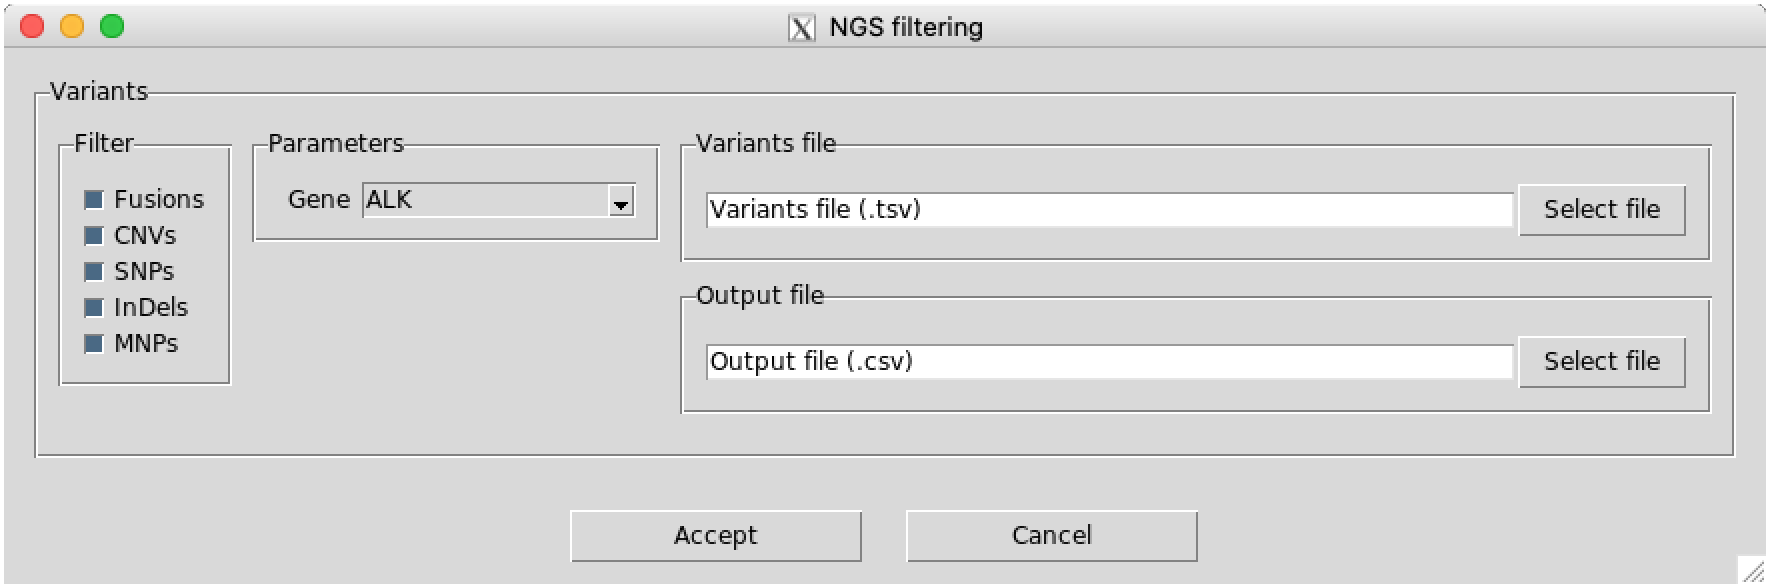
\includegraphics[width=\textwidth]{Images/chapter_4/GUI_1.png}
        \caption{Start screen. It allows selecting the type of variant\slash s to filter, the gene involved (ALK currently), as well as the source and output files. \\}
        \label{fig:GUI_1}
    \end{subfigure}
    \hfill
    \begin{subfigure}{0.47\textwidth}
        \centering
        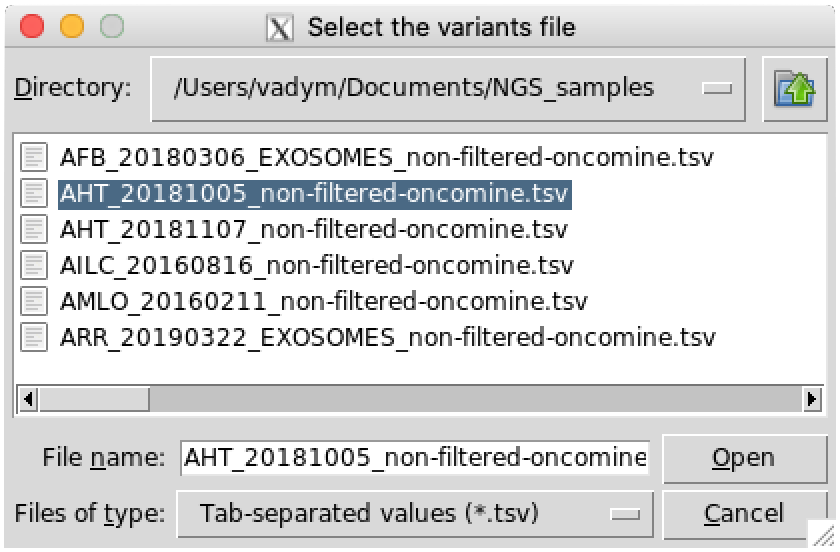
\includegraphics[width=\textwidth]{Images/chapter_4/GUI_2.png}
        \caption{Pop-up window for selecting the \textit{.tsv} source file containing raw variants.}
        \label{fig:GUI_2}
    \end{subfigure}
    \hfill
    \hfill
    \begin{subfigure}{0.52\textwidth}
        \centering
        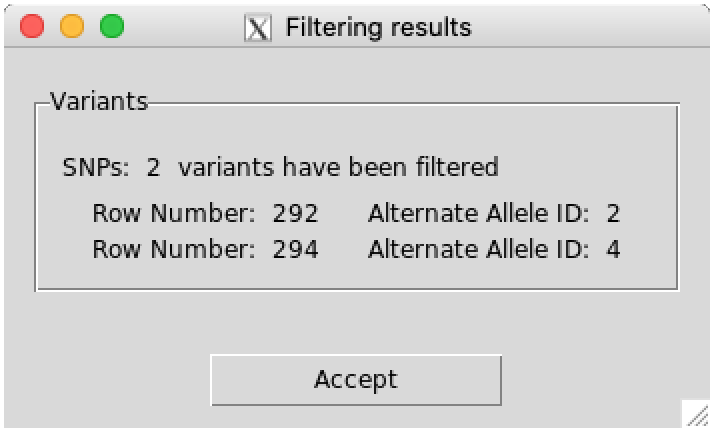
\includegraphics[width=\textwidth]{Images/chapter_4/GUI_3.png}
        \caption{Results screen showing 2 filtered SNPs, their $.tsv$ row number, and their alternate allele ID.}
        \label{fig:GUI_3}
    \end{subfigure}
    \hfill
    \caption{Implemented GUI showing the different display areas that appear throughout the filtering process.}
    \label{fig:GUI}
\end{figure}

The start screen (\autoref{fig:GUI_1}) has several options that allow some variability when proceeding with the filtering process. On the one hand, it is possible to select the filter\slash s to apply to the \textit{non-filtered-oncomine.tsv} file, as well as the gene to study. Currently, and as previously described, only the ALK gene has been addressed. On the other hand, the user can select both the source and output files through a pop-up screen, which is shown in \autoref{fig:GUI_2}. In case the output file does not exist, the program creates it automatically.

Finally, to fully characterize the variants that have passed a particular filter, the results are displayed specifying the mutation type, the row number of the variants in the \textit{non-filtered-oncomine.tsv} file, and the identifier of the alternate allele (\autoref{fig:GUI_3}). Simultaneously, each of the identified variants is appended to the $.csv$ output file along with its main characteristics.

It should also be noted that several additional screens have been implemented to offer the end-user information on the progress of the filtering process, on any errors that may have occurred during it, and on the non-identification of any variant of interest by the algorithm.

\section{Performance of the Developed Algorithm}

% Paper nuevo
% In order to increase sensitivity for the detection of somatic mutations in ALK locus we developed an algorithm designed to this aim. To do so, all ALK variants present in non-filtered-oncomine.tsv file were analyzed by dPCR. In total, 25 variants in ALK locus detected in 22 samples were analyzed by dPCR.  Considering the gold standard the dPCR results and assuming a prevalence of ALK mutations of 20%, the sensitivity, specificity, positive predictive value and negative predictive value of the designed algorithm were 77.8%, 76.5%, 45.3% and 93.2%, respectively (Table 2). Noteworthy, the oncomine variants filter v5.10 only detected ALK mutations in 3 patients (Table 3).


\section{Utility}

% A key benefit for physicians is the serial use of digital PCR to monitor one or more driver mutations throughout treatment to determine response and recurrence since the level of mutated DNA found in liquid biopsies has been found to reflect the size of the tumor(s). It is also possible to use NGS to track progress; however, in these cases it is less practical due to cost and longer turnaround time.


